\documentclass[letterpaper,10pt]{article}

\usepackage{titling}
\usepackage{listings}
\usepackage{url}
\usepackage{setspace}
\usepackage{subfig}
\usepackage{sectsty}
\usepackage{pdfpages}
\usepackage{colortbl}
\usepackage{multirow}
\usepackage{multicol}
\usepackage{relsize}
\usepackage{amsmath}
\usepackage{wasysym}
\usepackage{fancyvrb}
\usepackage{amssymb}
\usepackage{ifsym}
\usepackage{amsmath,amssymb,amsthm,graphicx,xspace}
\usepackage[titlenotnumbered,noend,noline]{algorithm2e}
\usepackage[compact]{titlesec}
\usepackage{XCharter}
\usepackage[T1]{fontenc}
\usepackage{tikz}
\usetikzlibrary{arrows,automata,shapes,trees,matrix,chains,scopes,positioning,calc}
\tikzstyle{block} = [rectangle, draw, fill=blue!20, 
    text width=2.5em, text centered, rounded corners, minimum height=2em]
\tikzstyle{bw} = [rectangle, draw, fill=blue!20, 
    text width=4em, text centered, rounded corners, minimum height=2em]

\definecolor{namerow}{cmyk}{.40,.40,.40,.40}
\definecolor{namecol}{cmyk}{.40,.40,.40,.40}

\let\LaTeXtitle\title
\renewcommand{\title}[1]{\LaTeXtitle{\textsf{#1}}}


\newcommand{\handout}[5]{
  \noindent
  \begin{center}
  \framebox{
    \vbox{
      \hbox to 5.78in { {\bf ECE356: Database Systems } \hfill #2 }
      \vspace{4mm}
      \hbox to 5.78in { {\Large \hfill #4  \hfill} }
      \vspace{2mm}
      \hbox to 5.78in { {\em #3 \hfill} }
    }
  }
  \end{center}
  \vspace*{4mm}
}

\newcommand{\lecture}[3]{\handout{#1}{#2}{#3}{Lecture #1}}
\newcommand{\tuple}[1]{\ensuremath{\left\langle #1 \right\rangle}\xspace}

\addtolength{\oddsidemargin}{-1.000in}
\addtolength{\evensidemargin}{-0.500in}
\addtolength{\textwidth}{2.0in}
\addtolength{\topmargin}{-1.000in}
\addtolength{\textheight}{1.75in}
\addtolength{\parskip}{\baselineskip}
\setlength{\parindent}{0in}
\renewcommand{\baselinestretch}{1.5}
\newcommand{\term}{Winter 2018}

\singlespace


\begin{document}

\lecture{ 28 --- More Recovery \& ARIES }{\term}{Jeff Zarnett}

\section*{Fuzzy Checkpointing}

Thus far when we have talked about creating a checkpoint assumes that we stop all execution, briefly, to take the snapshot. This sort of thing is not unheard of in programs, such as the ``stop the world'' garbage collector behaviour in Java. It might be, however, undesirable or even unacceptable: for a sufficiently large buffer it might take an usually long time. Therefore we would like to modify the checkpoint system to avoid having to halt all execution.

The term for a checkpoint that isn't such a clean division between here and there is called a \textit{Fuzzy Checkpoint}. A fuzzy checkpoint allows updates to start once the checkpoint has been created but before the modified buffer blocks are written to disk~\cite{fds}. There's still a pause in execution while the checkpoint is created, but that should be the fast part.

This does potentially present a problem: the checkpoint data is written to disk before the blocks are written and we could have a crash before all the blocks are written to disk. What do we do then? Keep track of the last completed checkpoint, and don't update the last completed checkpoint marker until all blocks have been output.

Note that even with fuzzy checkpoints, a block cannot be updated while it is being output to disk (although other blocks can be modified)~\cite{dsc}. Fuzzy checkpoints are more or less the standard approach in the real world because the alternatives take too long.

\section*{Recovering from Loss of Nonvolatile Storage}

The recovery routines considered so far are about booting the server up again after a crash or power failure or other temporary outage where nonvolatile storage is unaffected. But bad things will happen to even nonvolatile storage. So we need to take copies of the data to account for the fact that even supposedly nonvolatile storage is lost.

But how do we back up the database data? It is called a \textit{dump}. It is basically taking a copy of all the data. If we are doing it live, we require that no transactions are running and the steps are~\cite{dsc}:

\begin{enumerate}
	\item Write all log records currently in main memory to stable storage
	\item Write all buffer blocks to disk
	\item Copy the contents of the database to stable storage
	\item Note completion of the dump in the log
\end{enumerate}

The form the dump takes could be raw data, but there are tools in most database packages that exports the data as a SQL dump: it writes out the data description language (create table statements, for example) and insert table statements for the data. Such a dump can be used to copy the database from one system to another or migrate it from one database server to another.

The approach described above does have the obvious downside of needing to stop execution for a very long time. That is, however, not realistic. A tool that dumps the database like \texttt{mysqldump} takes a complete database dump, but it does so as a transaction: it gets a snapshot of the data at the time the dump is requested; further changes can still go on in the meantime but this transaction will be left running for as long as it takes (and it can be HOURS!).

An import will need to be run to get the data back into the database from the dump file if it was in SQL format. In the case of a loss of all data then it is imported into a fresh (empty) database; otherwise the previous (corrupt, partial, or otherwise problematic) data is dropped and it is replaced with the data from the import.

Exporting seems fairly easy from a technical perspective: just copy the data to the output file in the form of create table statements and then insert into statements. That works but there is a problem when importing. Tables are added and they have foreign key constraints. But how can you set up the key constraints if the other tables don't exist? And how can you insert the data for one table that references another without that other table having the data present as well?

There is some possibility to do a topological sort where you find a sequence of create table and add constraint statements, then one for insert statements... This is very difficult and potentially impossible depending on how your data is defined. The real answer is that when importing data via this method, integrity constraints are temporarily disabled to allow the file to be processed sequentially without any slowdowns.

Another way that backups tend to get taken is at the level outside of the database: the operating system. The data is ultimately stored somewhere on a volume (or volumes) in the database and the operating system can do things like shadow copies and image backups of the drives. Of course, the state that is stored to the disk at the time of the backup is what gets copied. If this is not a consistent state, some additional actions may be needed on startup to get things back to a consistent state.

\section*{ARIES}
In spite of sounding like the name of a NASA program to Mars or some such, the ARIES algorithm is a database recovery routine used by IBM. It relies on three main pillars: write-ahead logging, repeating history during redo, and logging changes when undoing something. The description of how ARIES works is all from~\cite{fds}.

The algorithm and the approach we have examined for recovery works and it produces the correct results, but it comes with some drawbacks and performance decreasing elements. ARIES is hopefully going to address it. ARIES is broken up into three phases: analysis, redo, and undo.

\paragraph{Analysis.} In the analysis phase, the goal is to figure out what pages in the buffer were dirty. We don't have the actual pages, of course, because the crash caused the loss of that data. However, e can determine the information based on the log data from the checkpoints: the dirty page table, transaction table, et cetera. During this phase a determination will also be made as to where to begin the redo phase.

\paragraph{Redo.} In the redo phase, updates from the log are done in the database. The normal recovery routine expects that we only redo committed transactions, but in ARIES we will try hard to skip unnecessary work: and only redo operations that are necessary.

\paragraph{Undo.} The last phase is the undo phase, and the log is scanned backwards and transactions that were active at the time of the crash are undone in reverse order. 

Every log has a LSN -- \textit{Log Sequence Number}; this is an incrementing counter that indicates the log record's address on disk; each number corresponds to a specific change of some transaction. Each data page stores the LSN of the most recent log record that changed that page. Log records are generated for updating a page, committing a transaction, aborting a transaction, undoing an update, and ending a transaction.  When an update is undone, a compensation log record is added; when a transaction ends, successfully or unsuccessfully, an end log record is written. 

The log structure has numerous fields, including the previous LSN for that transaction, the transaction ID, and what type of transaction is being written. The LSN can link (in reverse order) the log records for the same transaction. Other fields in each log record might include where to find the item (page, offset, etc), as well as the before and after values.

To perform a recovery, we need the log as well as the \textit{transaction table} and \textit{dirty page table}, both of which are maintained by the transaction manager. The transaction table lists the various transactions in progress. Similarly, the dirty page table contains the pages that are dirty (shocking, I know). These are lost when a crash occurs but are rebuilt when the system comes back online, obviously by looking at the log data. Thos tell us about what information is in progress.

To take a checkpoint, some steps are the same as the regular checkpoint process: a begin-checkpoint entry is added to the log, the checkpoint is written, and then the end-checkpoint entry is added. Alongside the end-checkpoint entry, the data for the transaction table and dirty page table are written to the log as well. The last step is to add the LSN of the begin-checkpoint entry to a special file. This special file just marks the location of the last successfully completed checkpoint operation and it will be checked during recovery so we know where our last checkpoint is. Note that fuzzy checkpointing is used so the cost of writing all this data out is not so high. If a crash occurs during the checkpoint process, the special file will not yet have been updated so we will resume from the earlier point.

After a crash occurs, the recovery process begins. The first thing is to use the special file just mentioned to find the place in the log where the process starts. This is where the analysis phase begins: start with the begin-checkpoint entry and keep moving until the end of the log (with stops along the way). 

When the end-checkpoint entry is found, the transaction table and dirty page table are read into memory. Their content will be altered in memory as log processing continues: if a transaction $T$ was in progress at the time of the end of the checkpoint and we then encounter an end-transaction record for $T$ then we know that it completed (successfully or otherwise) and we can remove $T$ from the memory list of transactions in progress. If instead we found a transaction $T$ that was not in the in-progress transaction list at the time of the end checkpoint, we will add it to the transaction table. 

Whether the transaction was known or not before encountering an operation involving it, anything other than an end-transaction statement will result in updating the LSN for that transaction in our records. If the transaction's operation results in a change to a page $P$, then $P$ is added to the dirty page list (if not already present) and the LSN field for $P$ is updated as well. 

At the conclusion of the analysis phase, the transaction table and dirty page table have all the information necessary to make the changes to return the system to a consistent state.

The redo phase begins: to avoid having to do anything unnecessary, no changes are done that have already been saved to disk. It is easy enough to tell which changes are done: look at the dirty page table, and find the smaller LSN, which we will call $M$. Anything before that is already done, so we can skip over records in the log that have a LSN smaller than $M$ (because they are already done or overwritten in memory). Redo starts then at the LSN equal to $M$ and scans forward to the log. 

For each change, consider whether the page $P$ is in the dirty page table. If it is not, then the change is already on disk. If $P$ is in the dirty page table, but has a LSN larger than the current change, the change is already written to disk and does not need to be reapplied. If $P$ is in the dirty page table but does not have a larger LSN,, page $P$ is read from disk and the disk stored version is checked; if the LSN is larger than that of the operation being performed then we can skip this operation.  If none of those conditions led to skipping the operation then the redo is applied. 

That concludes the redo phase; at this point the database is in the exact state it was in at the time of the crash, but the state is not consistent. There are still uncompleted transactions with partial progress that need to be rolled back. That is the job of the undo phase.

The log is scanned backwards from the end and each operation by a transaction in the ``undo set'' is undone by entering a compensating transaction record. The undo set is all transactions that were in progress at the time of the last checkpoint, plus all those that started after the checkpoint, subtracting those that finished before the crash (regardless of whether they were in progress at the checkpoint). 

Once that is done then the database is restored to a consistent state and normal operations may resume. 

Let us now do a simple example of how ARIES works from~\cite{fds}. Let us assume we have three transactions $T_{1}, T_{2}, T_{3}$. $T_{1}$ updates page $C$, $T_{2}$ updates $B$ and $C$, and $T_{3}$ updates $A$. We then have a crash occur, and the state of the system is as shown in the two diagrams below:

\begin{center}
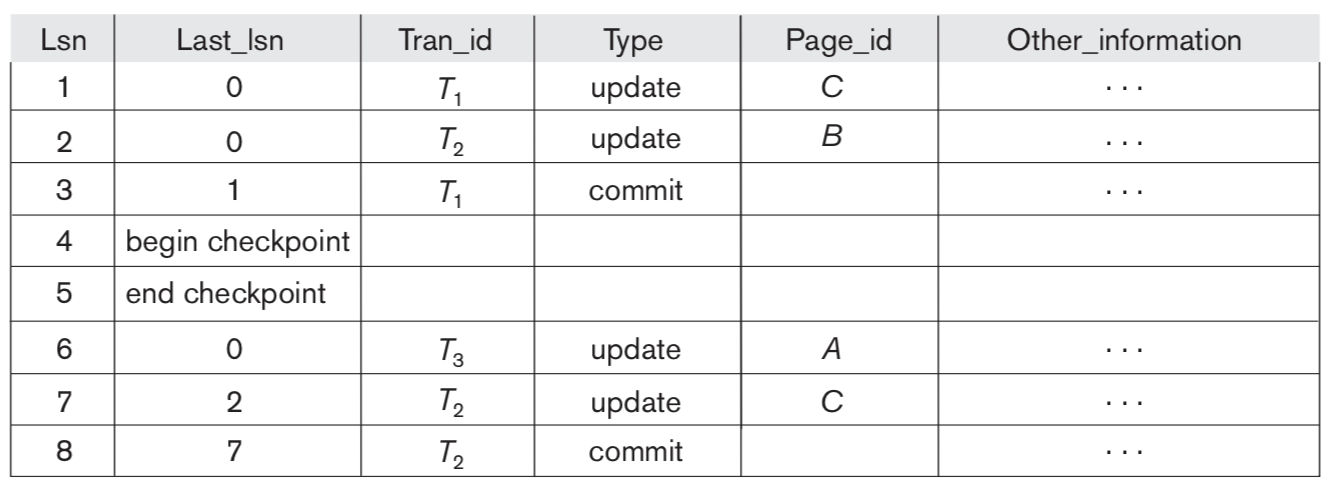
\includegraphics[width=0.85\textwidth]{images/aries-1}\\
The log at the point of the crash~\cite{fds}.
\end{center}

\begin{center}
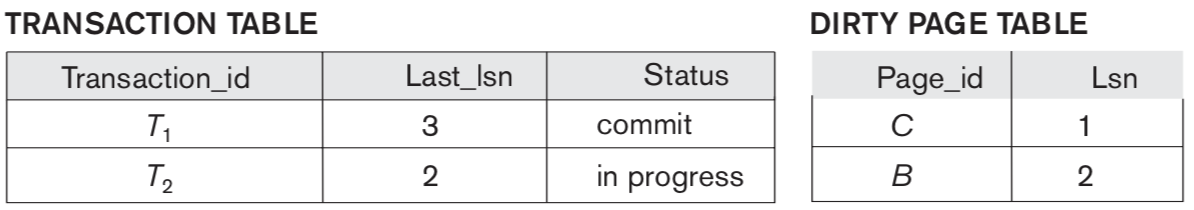
\includegraphics[width=0.85\textwidth]{images/aries-2}\\
Transaction Table and Dirty Page Table at the time of the crash~\cite{fds}.
\end{center}

With this information in hand we may begin to execute the algorithm. The first step is the analysis phase. The first step is to go to the most recently completed checkpoint. That so happens to be at LSN 4. So analysis moved from there forward. 

LSN 5 is the end checkpoint statement so it contains the transaction and dirty page tables. In LSN 6, transaction $T_{3}$ is found and added to the the list of transactions in progress. LSN 7 doesn't tell us anything new, but LSN 8 tells us that the transaction $T_{2}$ has committed. So the analysis phase is complete and the result is shown below. It's worth noting that transactions $T_{1}$ and $T_{2}$ have status ``commit'' but still appear in there -- because the pages they have updated have not been written to disk. 

\begin{center}
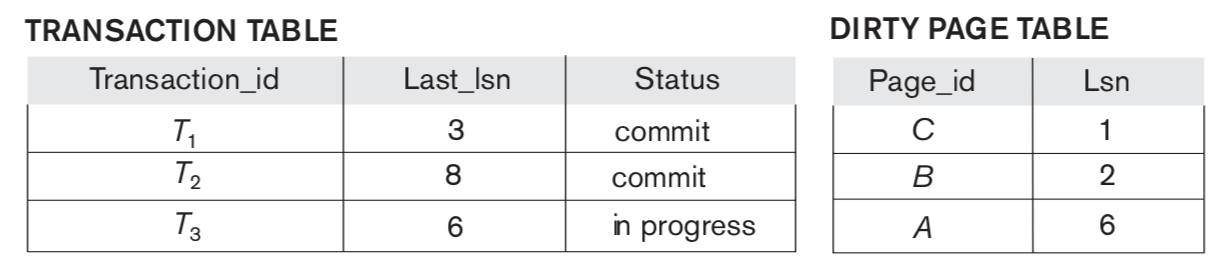
\includegraphics[width=0.85\textwidth]{images/aries-3}\\
Transaction Table and Dirty Page Table after analysis~\cite{fds}.
\end{center}

Then it is time for the redo phase: the smaller LSN in the dirty page tables is 1 (page $C$) so that's where we start the redo process. LSNs 1, 2, 6, and 7 want to update pages that have higher LSNs than the updates, so no need to repeat that update.

The undo phase here is very simple: the only thing to undo is the operations of $T_{3}$. We go backwards and the only log entry we need to undo is LSN 6. At that point we are all done.


\section*{Remote Backups}

Somewhat related to the idea of recovering our database if we have a crash is the idea of an online backup: a second copy of the database standing by to take over if the primary one should go down (whether through a crash or by losing network connection). The second copy is certainly on different hardware, and should more likely be located at a different physical location. 

By moving it to a different physical location, of course, that adds some latency to the connection: it takes nontrivial time for data to be transferred from the primary to the backup location. And that means that a strategy for keeping these in sync is necessary, but there are other considerations:

\paragraph{Detecting failure.} As you might imagine, the backup system needs to detect that the primary has failed so it knows when to take over. Ideally there are multiple independent communication lines between the primary and the backup so that the failure of any single one is not mis-detected as a failure of the primary system~\cite{dsc}.

\paragraph{Taking over.} Suppose a real failure is detected and the primary has crashed. In the meantime, the backup does the job of the primary. If the first system comes back online, it could be the new backup or it could retake the role of primary. Either way, it needs to get caught up on the things that have happened in the meantime. Once both systems are back online, the redo logs can be sent to the system that is behind to get it caught up~\cite{dsc}.

\paragraph{Making extra sure.} In this sort of configuration, is a transaction really committed until it has reached the backup site? It turns out we get a choice of how much we are willing to tolerate~\cite{dsc}:

\begin{itemize}
	\item \textbf{One-Safe}: If the transaction has been written to stable storage at the primary location. If there is a crash at the primary before that transaction has made it to the secondary location, then it may appear to be lost. When the primary site comes back, it may happen that in the meantime there has been an incompatible change made only on the secondary. Imagine you book seat 4A on the primary system and it crashes; someone else then books 4A on the secondary system. Who gets the seat? This is something that may require humans to sort out.
	\item \textbf{Two-Very-Safe}: A transaction is only committed once it is in both the primary and backup stable storage... which means that no transactions can be executed if one site is down.
	\item \textbf{Two-Safe}: A transaction is only committed once it is in both the primary and backup stable storage... if both are up; otherwise it is the same as one-safe: the primary suffices. 
\end{itemize}

Either two-safe or two-very-safe necessarily comes with a performance penalty: when the transaction is committed the changes must be propagated to the other server (if up) to consider the transaction fully done.

We're not limited to only two-safe protocols, of course. We could insist on an $n$-safe protocol where we have some additional replica servers and we consider the transaction done only when all $n$ servers have completed the transaction. The cost of having $n$ servers contain the data is really not much higher than the cost of having two: we have to send the data out and wait for confirmation, but much of this can be done in parallel.

But if we are going to be sending data out to multiple databases... are we sure they agree? We will need to come back to this subject next...

\bibliographystyle{alphaurl}
\bibliography{356}


\end{document}
